\begin{pastexam}[label={px:ncku-110-ee-ds-03}]{成大電機所 110 學年度 第 3 題}
（手算追蹤）

Read the following data in the given order: \quad (30 \%)
\begin{center}55, 45, 25, 35, 85, 95, 65, 75, 105, 15\end{center}
\begin{enumerate}[label=(\alph*)]
\item If you create a max heap for them, what will be the value in root? \hfill (10 \%)
\item If you create a 2-3 tree for them, what will be the value in root? \hfill (10 \%)
\item If you create an AVL tree for them, what will be the value in root? \hfill (10 \%)
\end{enumerate}
\end{pastexam}

\begin{pastsoln}
答案：(a) $105$；(b) $65$；(c) $45$。

三個小題分屬資結書第~8、11、10~章，追蹤最長的是 (b) 的 2-3 樹，本題放在第~11~章。 都照讀入的順序
一個一個插入。

\textbf{(a)} 最大堆積的根一定是全部資料的最大值，不管是逐一插入還是由下而上建，根都是 $105$。 （逐一
插入時，$105$ 插入後會一路往上換到根，之後插入的 $15$ 比它小，不會再換上去。）

\textbf{(b)} 2-3 樹（資結書第~11.1.3~節）：鍵都插在葉節點；節點滿了（變成 $3$ 個鍵）就分裂，中間的鍵往
上送到父節點，父節點也滿了就繼續往上，根分裂時樹長高一層。
\begin{center}
\small
\begin{tabular}{cl}
\toprule
插入 & 之後的樹（$[\,]$ 是一個節點，括號裡是它的子節點） \\
\midrule
55 & $[55]$ \\
45 & $[45, 55]$ \\
25 & $[25, 45, 55]$ 分裂，$45$ 上升：$[45]([25], [55])$ \\
35 & $[45]([25, 35], [55])$ \\
85 & $[45]([25, 35], [55, 85])$ \\
95 & 葉 $[55, 85, 95]$ 分裂，$85$ 上升：$[45, 85]([25, 35], [55], [95])$ \\
65 & $[45, 85]([25, 35], [55, 65], [95])$ \\
75 & 葉 $[55, 65, 75]$ 分裂，$65$ 上升，根變成 $[45, 65, 85]$ 又分裂，$65$ 上升成新根： \\
 & \quad $[65]\bigl([45]([25, 35], [55]),\ [85]([75], [95])\bigr)$ \\
105 & $[65]\bigl([45]([25, 35], [55]),\ [85]([75], [95, 105])\bigr)$ \\
15 & 葉 $[15, 25, 35]$ 分裂，$25$ 上升到 $[45]$： \\
 & \quad $[65]\bigl([25, 45]([15], [35], [55]),\ [85]([75], [95, 105])\bigr)$ \\
\bottomrule
\end{tabular}
\end{center}
\begin{center}
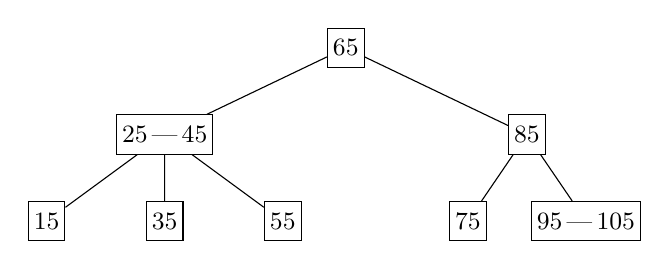
\begin{tikzpicture}[level distance=11mm,
  level 1/.style={sibling distance=46mm},level 2/.style={sibling distance=15mm},
  every node/.style={draw,rectangle,inner sep=2pt,minimum height=5mm,font=\small}]
\node {65}
  child {node {25\,|\,45} child {node {15}} child {node {35}} child {node {55}}}
  child {node {85} child {node {75}} child {node {95\,|\,105}}};
\end{tikzpicture}
\end{center}
根是 $65$。

\textbf{(c)} AVL 樹（資結書第~10.2.4~節）：
\begin{itemize}
\item $55$、$45$：$45$ 是 $55$ 的左子節點。
\item $25$：$55$ 的平衡因子 $+2$，新節點在左子節點的左邊，\textbf{LL 型}，在 $55$ 右旋，根變成 $45$（左 $25$、右 $55$）。
\item $35$：成為 $25$ 的右子節點；$25$ 是 $-1$、$45$ 是 $+1$，不轉。
\item $85$：成為 $55$ 的右子節點；$45$ 是 $0$，不轉。
\item $95$：成為 $85$ 的右子節點。 $55$ 的平衡因子 $-2$，新節點在右子節點的右邊，\textbf{RR 型}，在
$55$ 左旋：$85$ 取代 $55$（左 $55$、右 $95$）。 $45$ 是 $-1$。
\item $65$：$65 > 45$、$65 < 85$、$65 > 55$，成為 $55$ 的右子節點；$55$ 是 $-1$、$85$ 是 $+1$；$45$ 的
左子樹 $25$ 高度 $1$、右子樹 $85$ 高度 $2$（葉的高度算 $0$），是 $-1$，不轉。
\item $75$：成為 $65$ 的右子節點。 $65$ 是 $-1$；$55$ 左空、右高度 $1$，平衡因子 $-2$，新節點在 $55$ 的
右子節點 $65$ 的右邊，\textbf{RR 型}，在 $55$ 左旋：$65$ 取代 $55$（左 $55$、右 $75$）。 $85$ 左高 $1$、
右高 $0$，是 $+1$；$45$ 是 $-1$。
\item $105$：成為 $95$ 的右子節點；$95$ 是 $-1$、$85$ 是 $0$、$45$ 是 $-1$（左高 $1$、右高 $2$），不轉。
\item $15$：成為 $25$ 的左子節點；$25$ 是 $0$，高度仍是 $1$，$45$ 仍是 $-1$，不轉。
\end{itemize}
最後的樹：
\begin{center}
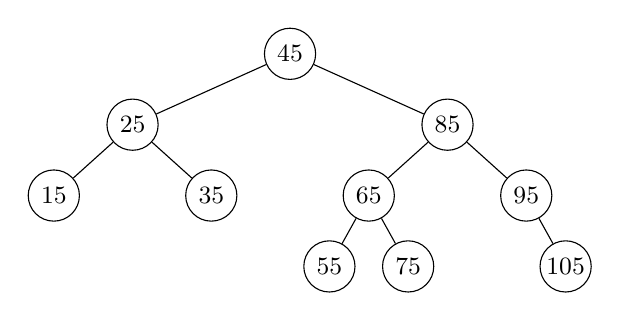
\begin{tikzpicture}[level distance=9mm,
  level 1/.style={sibling distance=40mm},level 2/.style={sibling distance=20mm},
  level 3/.style={sibling distance=10mm},
  every node/.style={circle,draw,inner sep=0pt,minimum size=6.5mm,font=\small}]
\node {45}
  child {node {25} child {node {15}} child {node {35}}}
  child {node {85} child {node {65} child {node {55}} child {node {75}}}
                   child {node {95} child[missing] child {node {105}}}};
\end{tikzpicture}
\end{center}
根是 $45$。 只有插入 $25$ 那一次的旋轉換過根，之後的旋轉都發生在右子樹裡面。
\end{pastsoln}
